\documentclass[aspectratio=169]{beamer}
% \documentclass[aspectratio=169, handout]{beamer}
 
\usepackage{pgffor}
\usepackage{algo}
\usepackage{sigmastyle}
% \usepackage{subcaption}

\usepackage[backend=biber,style=authoryear,defernumbers=true]{biblatex}
\addbibresource{refs.bib}

\newcommand{\pauseitem}{\onslide<+-> \item}

\DeclareCiteCommand{\footpartcite}[\mkbibfootnote]
  {\usebibmacro{prenote}}%
  {\usebibmacro{citeindex}%
   \setunit{\addnbspace}
   \printnames{labelname}%
   \setunit{\labelnamepunct}
   \printfield[citetitle]{title}%
   \newunit
   \printfield[]{year}}
  {\addsemicolon\space}
  {\usebibmacro{postnote}}

\newcommand{\ExpD}{\mathrm{Exp}}

\DeclareMathOperator{\pmap}{map}
\DeclareMathOperator{\pscan}{scan}
\DeclareMathOperator{\pfilt}{filter}
\DeclareMathOperator{\pgroup}{group}

\setbeamertemplate{blocks}[rounded]
% \setbeamercovered{transparent}
\usecolortheme{orchid}
\usetheme{sigma}

\title{Parallel Graph Algorithms: Connectivity and SSSP}
\author{Ian Chen}
\date{}

\institute{University of Illinois Urbana-Champaign}

% --------------------------------------------------------------------

% Begin document
\begin{document}

\begin{frame}
    \titlepage
\end{frame}

\begin{frame}{Problem Statements}
    \begin{itemize}
        \pauseitem Connectivity: given an (undirected) graph $G = (V, E)$:
        \begin{itemize}
            \pauseitem How many connected components does the graph have?
            \pauseitem What is the size of the largest connected component?
            \pauseitem WLOG, assume no isolated vertices
        \end{itemize}
        \pauseitem Single source shortest paths: given a (weighted, undirected) graph $G = (V, E)$ and source vertex $s \in V$:
        \begin{itemize}
            \pauseitem What is the (length of) shortest path from $s \to v$ for $v \in V$?
        \end{itemize}
    \end{itemize}
\end{frame}

\frame{\tableofcontents}

\section{Parallel Models}
\frame{\tableofcontents[currentsection]}

\begin{frame}{Parallel Model}
    \begin{itemize}
        \pauseitem Random-Access Machine (RAM) model:
        \begin{itemize}
            \pauseitem Standard model of manipulating words
        \end{itemize}
        \pauseitem Parallel RAM (PRAM) model:
        \begin{itemize}
            \pauseitem $P$ processors, typically $P = \poly(n)$
            \pauseitem Concurrent Read Concurrent Write (CRCW)
        \end{itemize}
        \pauseitem Work: number of elementary operations
        \pauseitem Depth: max sequence of dependent operations
        \pauseitem Brent's Theorem: PRAM algorithm takes $O(\frac{W}{P} + D)$ time
        \pauseitem $P^* = \frac{W}{D}$ maximum parallelism of an algorithm
    \end{itemize}
\end{frame}

\begin{frame}{Concurrency Primitives}
    \begin{itemize}
        \pauseitem $\pmap$: apply a function $f$ onto each element of an array $A$
        \begin{itemize}
            \pauseitem $O(n)$ work, $O(1)$ depth
        \end{itemize}
        \pauseitem $\pscan$: given binary operation $\oplus$ (associative with identity), return new array $B_i = \bigoplus_{i \le j} A_i$
        \begin{itemize}
            \pauseitem $O(n)$ work, $O(\log n)$ depth
        \end{itemize}
        \pauseitem $\pfilt$: apply predicate $f$ onto each element of an array, and return new array with only true flags
        \begin{itemize}
            \pauseitem $O(n)$ work, $O(\log n)$ depth
        \end{itemize}
        \pauseitem $\pgroup$: given equality test $f$, reorder elements such that all equal elements are contiguous
        \begin{itemize}
            \pauseitem $O(n)$ work, $O(\log n)$ depth \footpartcite{gu15-06}
        \end{itemize}
    \end{itemize}
\end{frame}

\section{Graph Connectivity}
\frame{\tableofcontents[currentsection]}

\begin{frame}{Parallel BFS}
    \begin{algo}
        \textul{\textsc{ParallelBFS}(undirected graph $G = (V, E)$, source vertex $s \in V$)}: \+
        \\ $X \gets \set{s}$ active set
        \\ $F \gets N(X)$ frontier
        \\ \textbf{while} $\abs{F} > 0$:
        \+ \\ $X \gets X \cup F$; $F \gets N(X)$ \-
    \end{algo}
    \vspace{\baselineskip}

    \begin{itemize}
        \pauseitem Parallel BFS finds connected component of a source
        \pauseitem Iterate until visit every vertex in the graph
        \pauseitem $O(\Delta \log n)$ time where $\Delta$ sum of diameters of each component
    \end{itemize}
\end{frame}

\begin{frame}{Random Mating}
    \begin{itemize}
        \pauseitem Generate (asymmetric) stars with coin flips (tails and heads)
        \pauseitem A vertex is contracted if it is a tail and some adjacent node is head
        \begin{itemize}
            \pauseitem $P(v \text{ contracted}) = \frac{1}{2} \times (1 - 2^{-\deg(v)}) \ge \frac{1}{4}$
        \end{itemize}
        \pauseitem $O(\log n)$ iterations $\implies$ $O(m \log n)$ work and $O(\log^2 n)$ depth
    \end{itemize}

    \onslide<+->
    \vspace{\baselineskip}
    \begin{algo}
        \textul{\textsc{CountCcRandomMating}($G = (V, E)$)}: \+
        \\ if $E = \emptyset$, return $\abs{V}$
        \\ $\pmap(\operatorname{coinflip}, V)$
        \\ $E' \gets \pgroup$ edges from $T \to H$; reduce to at most one element
        \\ Contract all edges in $E'$
    \end{algo}
\end{frame}

\begin{frame}{Connectivity via Low Diameter Decompositions}
    \begin{itemize}
        \pauseitem BFS is work efficient but can be sequential on large-diameter graphs
        \pauseitem Contractions are depth efficient but cost additional work
        \pauseitem Let $\textsc{Ldd}(G) \subset G$ cover $O(m)$ edges and has ``low'' diameter.
        \pauseitem Contracting componentsd of LDD leads to efficient algorithm \footpartcite{shun14-06}
    \end{itemize}

    \vspace{\baselineskip}
    \begin{algo}
        \textul{\textsc{Cc}($G = (V, E)$)}: \+
        \\ if $E' = \emptyset$, return $V$
        \\ $L \gets \textsc{CcBfs}(\textsc{Ldd}(G))$
        \\ $L' \gets \textsc{Cc}(\textsc{Contract(G, L)})$
        \\ Return $\textsc{Relabel}(L, L')$
    \end{algo}
\end{frame}

\begin{frame}{Random Shift LDD}
    \begin{itemize}
        \pauseitem Start a BFS from multiple sources
        \pauseitem Partition nodes based on nearest source
        \pauseitem $u$ promotes itself to a seed at time $T_u$, if not visited
    \end{itemize}
\end{frame}

\begin{frame}{Random Shift LDD}
    \centering
    \foreach \n in {1,...,5} {
            \only<\n|handout:0>{
                \begin{figure}
                    \includegraphics[height=0.68\textheight]{figs/ldd_frame_000\n.pdf}
                    \caption{
                        \textbf{Low Diameter Decomposition with Random Shifts}:
                        $100 \times 100$ grid graph.
                        Colors represent clusters (gray unclustered).
                        Using $\lambda = 25$.
                    }
                \end{figure}
            }
        }
    \only<6>{
        \begin{figure}
            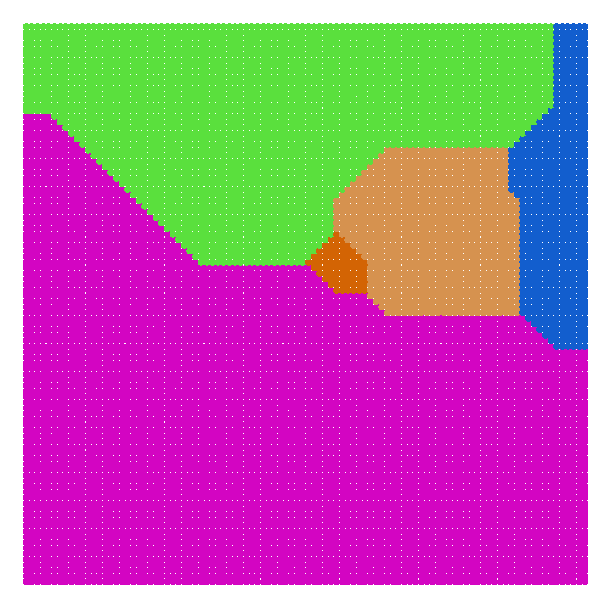
\includegraphics[height=0.68\textheight]{figs/ldd_frame_0006.pdf}
            \caption{
                \textbf{Low Diameter Decomposition with Random Shifts}:
                $100 \times 100$ grid graph.
                Colors represent clusters (gray unclustered).
                Using $\lambda = 25$.
            }
        \end{figure}
    }
\end{frame}

\begin{frame}{Random Shift LDD}
    \begin{itemize}
        \pauseitem What conditions do we want on $T_u$?
        \begin{itemize}
            \pauseitem $T_u$ and $T_u^{(k)}$ are independent
            \pauseitem $T_u \le O(\log n)$ with high probability, for low diameter
            \pauseitem $T_u^{(2)} - T_u^{(1)} > T_u^{(3)} - T_u^{(2)} > \ldots$, for low ``contention''
        \end{itemize}
        \pauseitem $T_u \sim C - \ExpD(\lambda = \frac{1}{2})$ for some constant $C$
        \pauseitem Find components via nearest neighbor $d_\delta(u, v) = T_u + d(u, v)$ \footpartcite{miller13-07}
    \end{itemize}

    \begin{algo}
        \textul{\textsc{Ldd}($G = (V, E)$)}: \+
        \\ Form $G'$ with additional vertex $s$
        \\ Add edges $su$ with weight $-\delta_u$ for each $u \in V$
        \\ Return $\textsc{Bfs}(G')$
    \end{algo}
\end{frame}

\begin{frame}{Recall: Exponential Distribution}
    \begin{itemize}
        \pauseitem Let $X_1, \ldots, X_n \overset{iid}{\sim} \ExpD(p)$, $X^{(k)} = X_{i_k}$ be the $k$-th order statistic:
        \pauseitem $P(X_i > t) = e^{-\lambda t}$, $E(X_i) = \frac{1}{\lambda} = 2$
        \pauseitem $P(X_i > s + t \mid X_i > s) = P(X_i > t) = e^{- \beta t}$
        \pauseitem $X^{(k+1)} - X^{(k)} \sim \ExpD((n - k - 1) \lambda)$
        \begin{align*}
            X_{i_{k+1}} - X_{i_k} & = P( X_{i_{k+1}}, \ldots, X_{i_n} > t + X_{i_k} \mid X_{i_{k+1}}, \ldots, X_{i_n} > X_{i_k}) \\
                                  & = P(X_{i_{k+1}}, \ldots, X_{i_n} \ge t)                                                      \\
                                  & = (e^{- \lambda t})^{n - k - 1} = e^{- ((n - k - 1) \lambda) t }
        \end{align*}
    \end{itemize}
\end{frame}

\begin{frame}[allowframebreaks]{Analysis}
    \begin{lemma}
        Let $[u] = \argmin_{v \in V} d_\delta(v, u)$.
        If $[u]$ = $[v]$, then $[u] = [w]$ for all $w$ on shortest path (in G) between $u$ and $v$.
    \end{lemma}

    \begin{proof}
        \begin{itemize}
            \item Let $u_0, u_1, \ldots, u_\ell$ be shortest path, $u_0 = u$ and $u_\ell = v$
            \item Induct on $u_i$ from $i=\ell$ to $i=0$
            \item For $i < \ell, u' \in V$, then $d_\delta(u, u_i) \le d_\delta(u', u_i)$, since
                  $$
                      d_\delta(u, u_i) + 1 \le d_\delta(u, u_{i+1})\le d_\delta(u', u_{i+1}) \le d_\delta(u', u_i) + 1
                  $$
            \item With probability 1, there are no ties, so equality only if $u = u'$
        \end{itemize}
    \end{proof}

    \begin{lemma}
        The diameter of each component is at most $O(\frac{\log n}{\lambda})$ w.h.p.
    \end{lemma}

    \begin{proof}
        \begin{itemize}
            \item $\Delta = \max_{u \in V} \min_{v \in V} d_\delta(v, u)$
            \item Fix any $u$, and let $w = \argmin_{v \in V} d_\delta(v, u)$
            \item $d(w, u) = d_\delta(w, u) + \delta_{w} \le d_\delta(u, u) + \delta_{w} = - \delta_{u} + \delta_{w} \le \delta_{w}$
            \item $$
                      P(\delta_w > 2 \frac{\log n}{\lambda}) = \exp{(- \lambda) \cdot 2 \frac{\log n}{\lambda}} = \frac{1}{n^2}
                  $$
            \item Union bound over all vertices, then $P(\Delta > 2 \frac{\log n}{\lambda}) \le \frac{1}{n}$
        \end{itemize}
    \end{proof}

    \begin{lemma}
        The expected number of edges $uv$ with $[u] \ne [v]$ is at most $\lambda m$.
    \end{lemma}

    \begin{proof}
        \begin{itemize}
            \item Fix an edge $uv$. We will show $P([u] \ne [v]) \le \lambda$.
            \item WLOG, say $d_\delta([u], u) \le d_\delta([v], v)$. Then, $d_\delta([u], u) \le d_\delta([v], u) + 1$
            \item Let $w \in V$ be the second min of $d_\delta(w, u)$: $d_\delta(w, u) \le d_\delta([v], u) + 1$
            \item Then, $Y = - d(w, u) + \delta_w$ and $X = - d([u], u) + \delta_{[u]}$ are the max and 2nd max of shifted geometric distribution
            \item $$
                      P(Y - X \le 1) = P(X^n_{(n)} - X^n_{(n-1)} \le 1) = 1 - e^{-\lambda} \le \lambda
                  $$
        \end{itemize}
    \end{proof}

    \begin{theorem}
        There exists an algorithm that solves connected components with $O(n+m)$ work and $O(\log^3 n)$ span with high probability.
    \end{theorem}

    \begin{proof}
        \begin{itemize}
            \item Find LDD with $\Delta = 2 \log n$ and $m/2$ edges w.h.p. ($\lambda = \frac{1}{2}$)
            \item BFS takes $O(\Delta \log n) = O(\log^2 n)$ depth and $O(n+m)$ work
            \item Work $W$ and depth $S$ recurrence (w.h.p.):
                  $$
                      W(n, m) = O(n+m) + W(n, m') \le O(n+m) + W(n, m/2) = O(n+m)
                  $$
                  $$
                      S(n, m) = O(\log^2 n) + S(n, m') \le O(\log^2 n) + S(n, m/2) = O(\log^3 n)
                  $$
        \end{itemize}
    \end{proof}
\end{frame}

\section{Single Source Shortest Paths}
\frame{\tableofcontents[currentsection]}

\begin{frame}{Bellman-Ford}
    \begin{itemize}
        \pauseitem Edge relaxation: $d(v) \le \hat{d}_k(v) \le \hat{d}_{k-1}(u) + w(u, v)$
        \pauseitem Nodes are settled in level-order of shortest paths tree $T_s$
        \pauseitem $O(h m)$ work, $O(h \log n)$ depth, where $h$ is height of $T_s$
    \end{itemize}

    \vspace{\baselineskip}
    \begin{algo}
        \textul{\textsc{BellmanFord}(undirected graph $G = (V, E)$, source vertex $s \in V$)}: \+
        \\ $\hat{d}(\cdot) \gets + \infty$, $\hat{d}(s) \gets 0$
        \\ for $k$ from $0$ to $\ldots$
        \+ \\ for $v_{jk} \in V$: \-
        \+ \+ \\ $\hat{d}_k(\cdot) \gets \min( \hat{d}_k(\cdot), \hat{d}_k(v_{jk}) + w(v_{jk}, \cdot) )$ \- \-
        \\ return $\hat{d}_k(\cdot)$
    \end{algo}
\end{frame}

\begin{frame}{Dijkstras}
    \begin{itemize}
        \pauseitem Edge relaxation\footnotemark: $d(v) \le \hat{d}(v) \le \hat{d}(u) + w(u, v)$
        \pauseitem Nodes are ``settled'' ($\hat{d}(v) = d(v)$) in distance-order
        \pauseitem $O(m \log n)$ work, $O(n \log n)$ depth
    \end{itemize}

    \vspace{\baselineskip}
    \begin{algo}
        \textul{\textsc{Dijkstras}(undirected graph $G = (V, E)$, source vertex $s \in V$)}: \+
        \\ $\hat{d}(\cdot) \gets + \infty$, $\hat{d}_0(s) \gets 0$
        \\ for $k$ from $0$ to $n-1$:
        \+ \\ $v_k \gets \argmin_{v \text{ not yet seen}} \hat{d}(v)$ \-
        \+ \\ $\hat{d}(\cdot) = \min( \hat{d}(\cdot), \hat{d}(v_k) + w(v_k, \cdot) )$ \-
        \\ return $\hat{d}(\cdot)$
    \end{algo}

    \footnotetext{We assume that all weights are at least $1$.}
\end{frame}

\begin{frame}{Focusing on depth}
    \begin{itemize}
        \pauseitem In worst case, $h = n-1$ (consider a linked list)
        \pauseitem What are some graphs where the height is much smaller?
        % TODO: make these figures instead of text
        \begin{itemize}
            \pauseitem Cliques
            \pauseitem Stars
        \end{itemize}
    \end{itemize}
\end{frame}

\begin{frame}{Focusing on depth}
    \begin{itemize}
        \pauseitem Barbarasi-Alberts (preferential-attachment) networks
    \end{itemize}

    \begin{center}
        \only<1|handout:0>{
            \begin{figure}
                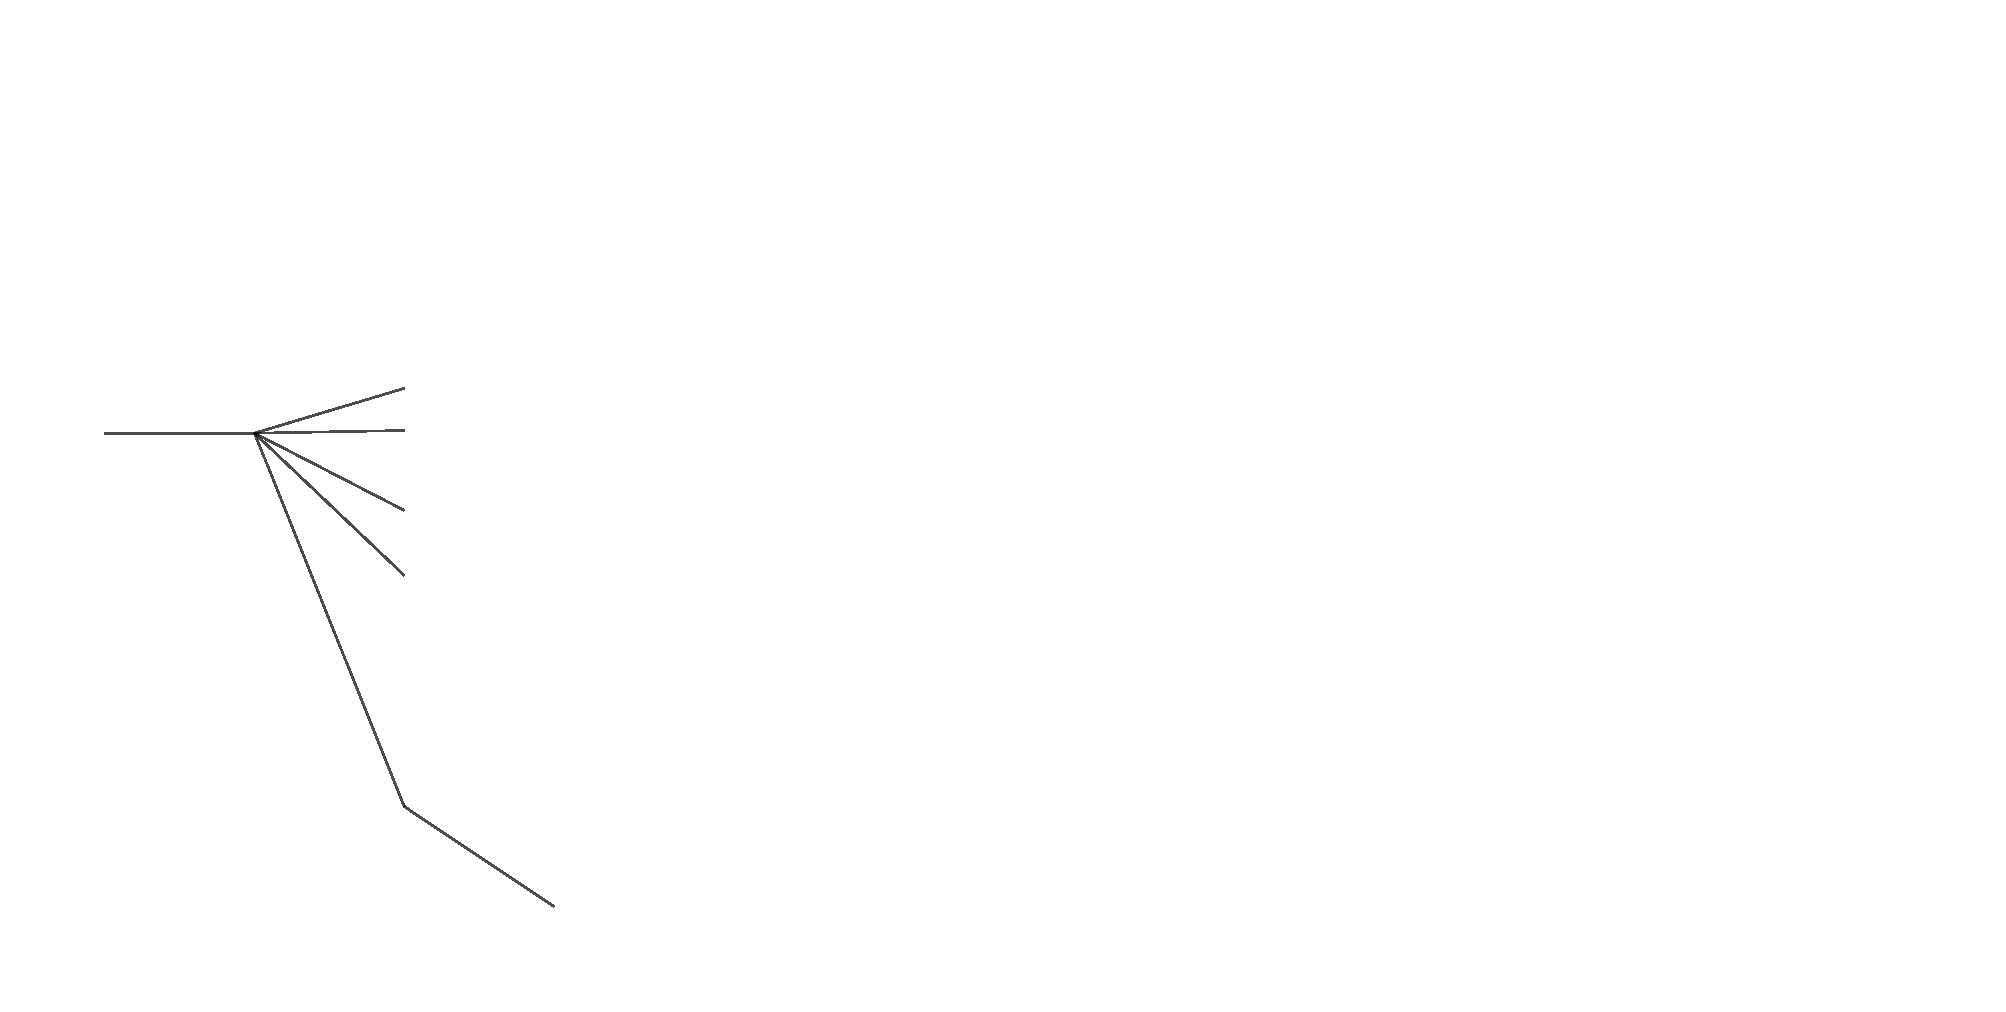
\includegraphics[width=0.75\textwidth]{figs/ba_tree_nodes_0008.pdf}
                \caption{\textbf{Growth of Barbarasi-Alberts network}: BA($n=8, m=1$)}
            \end{figure}
        }
        \only<2|handout:0>{
            \begin{figure}
                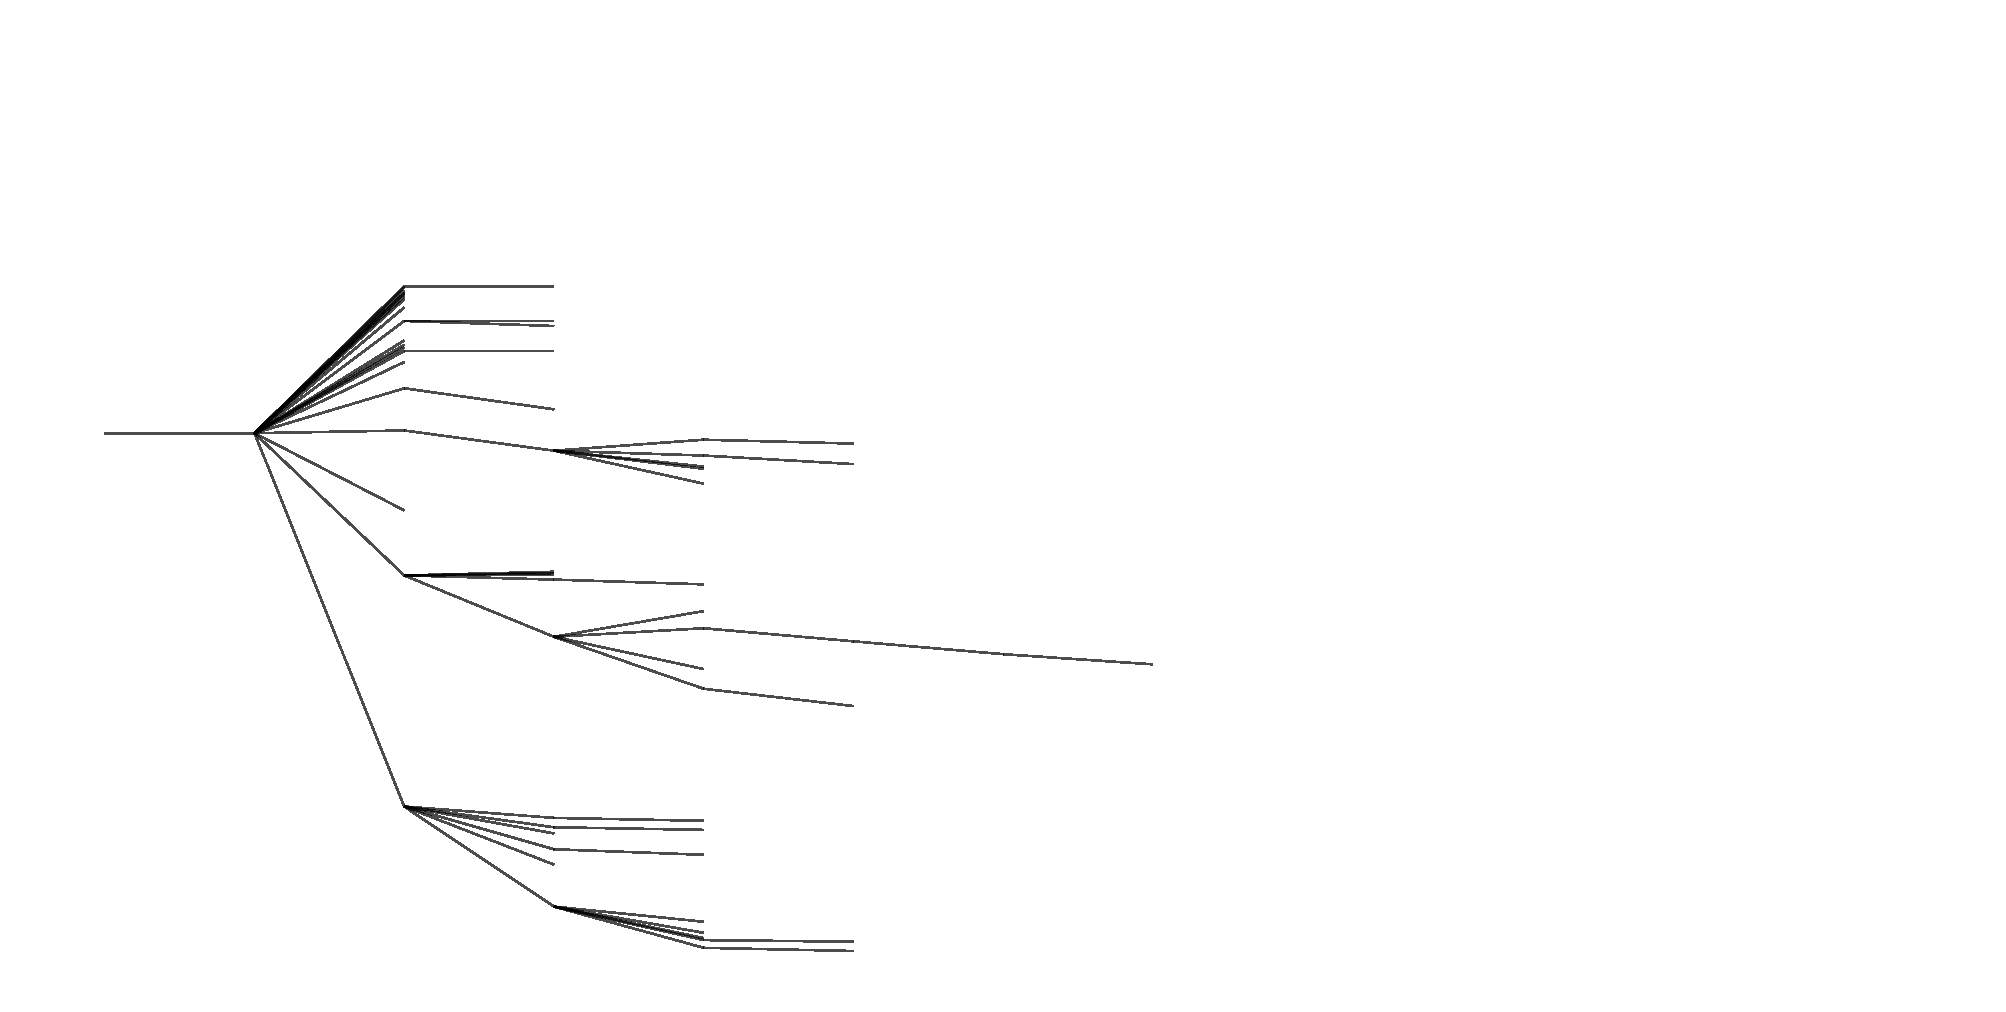
\includegraphics[width=0.75\textwidth]{figs/ba_tree_nodes_0064.pdf}
                \caption{\textbf{Growth of Barbarasi-Alberts network}: BA($n=64, m=1$)}
            \end{figure}
        }
        \only<3|handout:0>{
            \begin{figure}
                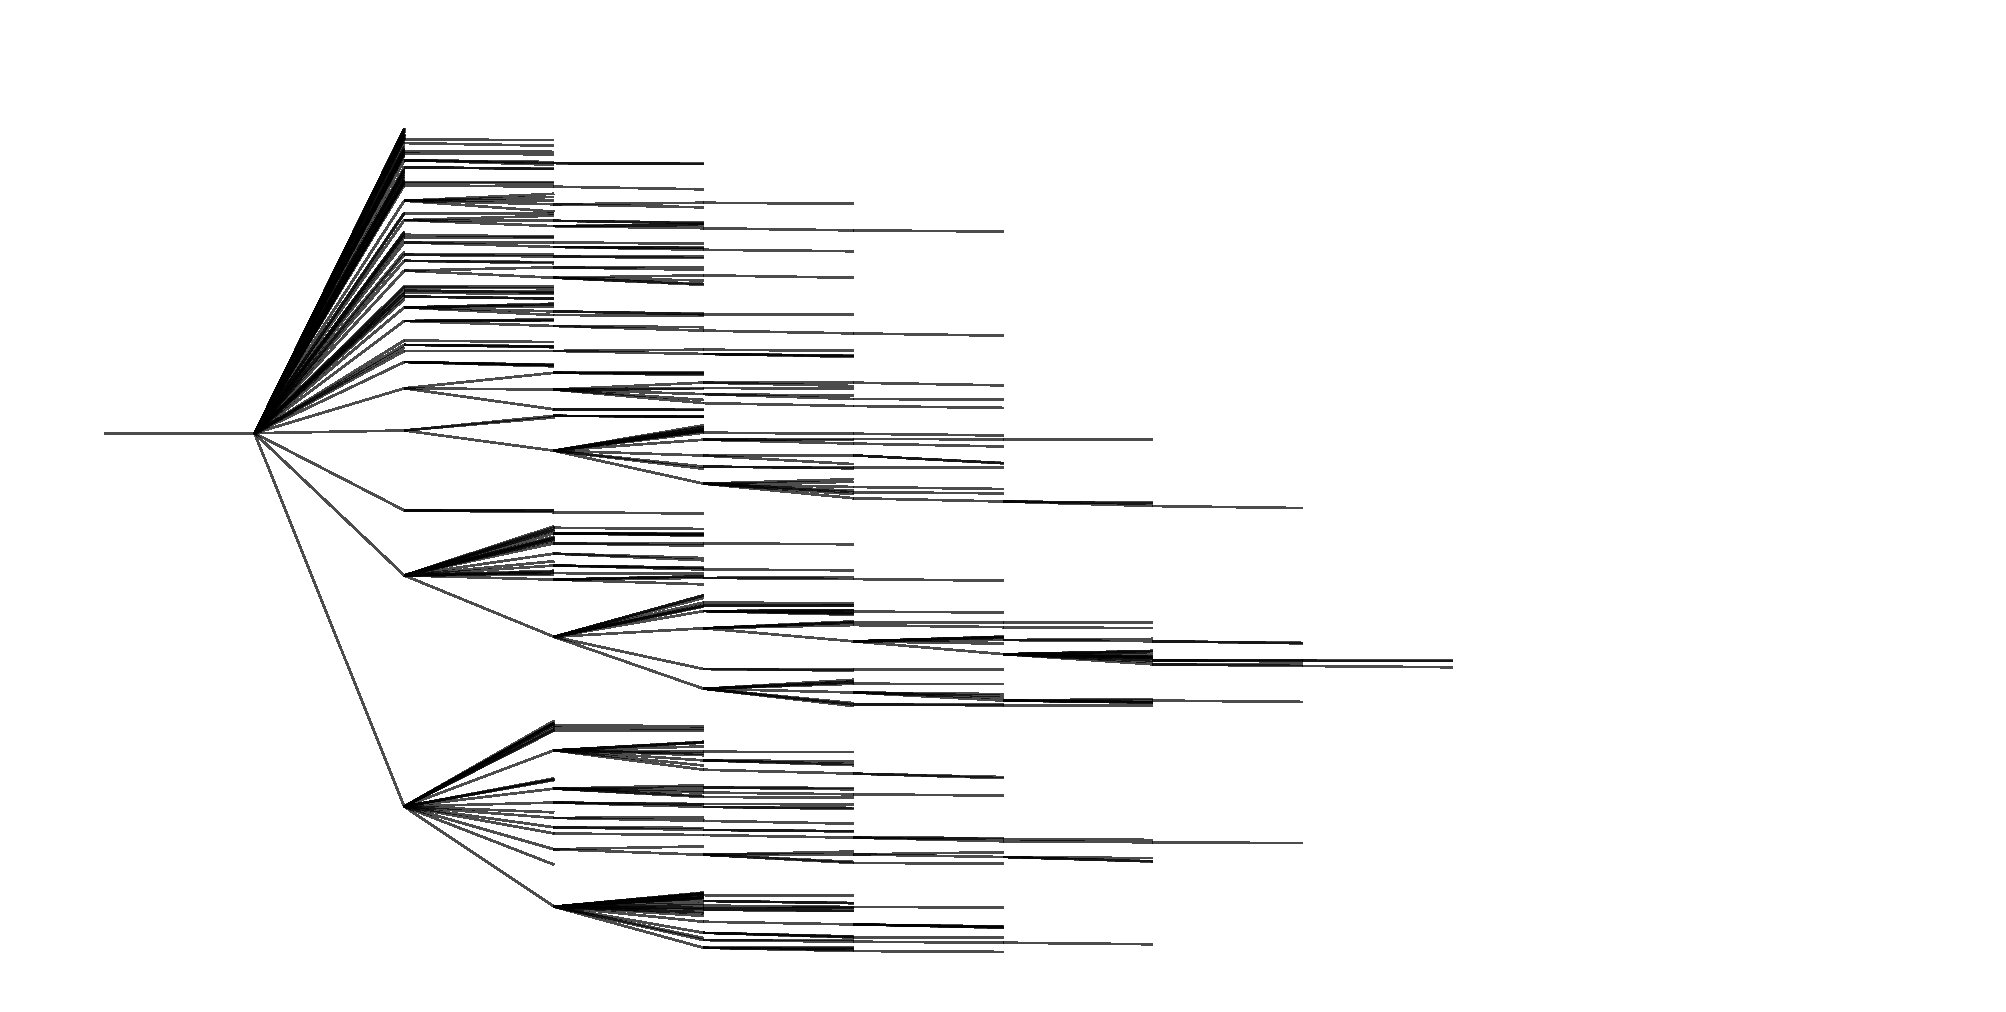
\includegraphics[width=0.75\textwidth]{figs/ba_tree_nodes_0512.pdf}
                \caption{\textbf{Growth of Barbarasi-Alberts network}: BA($n=512, m=1$)}
            \end{figure}
        }
        \only<4|handout:1>{
            \begin{figure}
                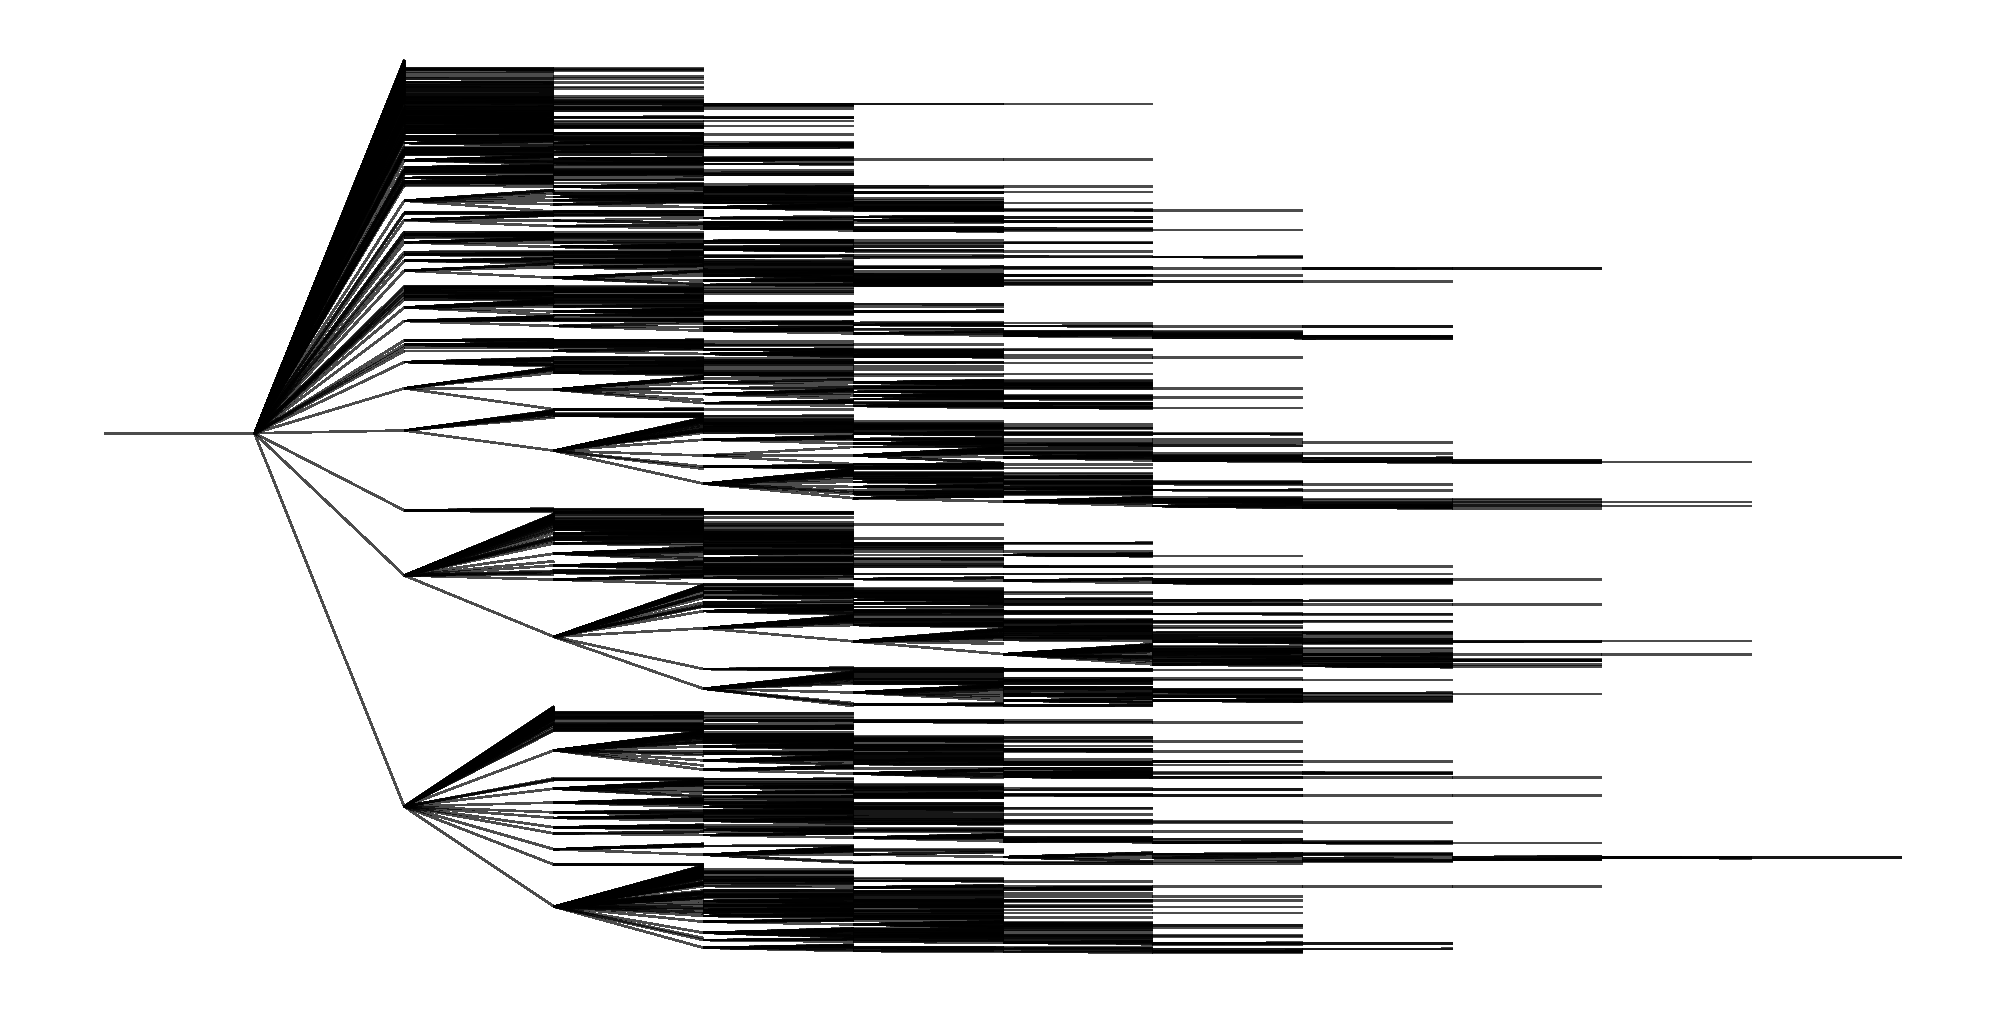
\includegraphics[width=0.75\textwidth]{figs/ba_tree_nodes_4096.pdf}
                \caption{\textbf{Growth of Barbarasi-Alberts network}: BA($n=4096, m=1$)}
            \end{figure}
        }
    \end{center}
\end{frame}

\begin{frame}{$(1,\rho)$ graphs}
    \only<1-11|handout:0>{
        \begin{itemize}
            \pauseitem $G$ is $(1,\rho)$ if every vertex is adjacent to its $\rho$ closest nodes
        \end{itemize}
    }
    \begin{center}
        \only<2|handout:0>{
            \begin{figure}
                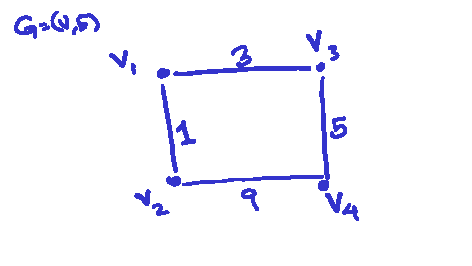
\includegraphics[width=0.8\textwidth, page=1]{figs/shortest_tree.pdf}
                \caption{\textbf{Converting $(1,2)$ graph}: Input graph with $n=m=4$}
            \end{figure}
        }
        \only<3|handout:0>{
            \begin{figure}
                \includegraphics[width=0.8\textwidth, page=2]{figs/shortest_tree.pdf}
                \caption{\textbf{Converting $(1,2)$ graph}: Shortest path tree of $v_1$}
            \end{figure}
        }
        \only<4|handout:0>{
            \begin{figure}
                \includegraphics[width=0.8\textwidth, page=3]{figs/shortest_tree.pdf}
                \caption{\textbf{Converting $(1,2)$ graph}: $v_1$ adjacent to $\rho$ closest nodes}
            \end{figure}
        }
        \only<5|handout:0>{
            \begin{figure}
                \includegraphics[width=0.8\textwidth, page=4]{figs/shortest_tree.pdf}
                \caption{\textbf{Converting $(1,2)$ graph}: Shortest path tree of $v_2$}
            \end{figure}
        }
        \only<6|handout:0>{
            \begin{figure}
                \includegraphics[width=0.8\textwidth, page=5]{figs/shortest_tree.pdf}
                \caption{\textbf{Converting $(1,2)$ graph}: $v_2$ not adjacent to $\rho$ nearest nodes}
            \end{figure}
        }
        \only<7|handout:0>{
            \begin{figure}
                \includegraphics[width=0.8\textwidth, page=6]{figs/shortest_tree.pdf}
                \caption{\textbf{Converting $(1,2)$ graph}: Shortcut $v_2v_3$ with weight $4$}
            \end{figure}
        }
        \only<8|handout:0>{
            \begin{figure}
                \includegraphics[width=0.8\textwidth, page=7]{figs/shortest_tree.pdf}
                \caption{\textbf{Converting $(1,2)$ graph}: Shortest path tree of $v_3$}
            \end{figure}
        }
        \only<9|handout:0>{
            \begin{figure}
                \includegraphics[width=0.8\textwidth, page=8]{figs/shortest_tree.pdf}
                \caption{\textbf{Converting $(1,2)$ graph}: $v_3$ is adjacent to $\rho$ closest nodes}
            \end{figure}
        }
        \only<10|handout:0>{
            \begin{figure}
                \includegraphics[width=0.8\textwidth, page=9]{figs/shortest_tree.pdf}
                \caption{\textbf{Converting $(1,2)$ graph}: Shortest path tree of $v_4$}
            \end{figure}
        }
        \only<11|handout:0>{
            \begin{figure}
                \includegraphics[width=0.8\textwidth, page=10]{figs/shortest_tree.pdf}
                \caption{\textbf{Converting $(1,2)$ graph}: Shortcut $v_4v_1$ with weight $8$}
            \end{figure}
        }
    \end{center}
    \only<12>{
        \begin{itemize}
            \pauseitem $G$ is $(1,\rho)$ if every vertex is adjacent to its $\rho$ closest nodes
            \pauseitem Every $G$ is a $(1,1)$ graph
            \pauseitem Can check whether a graph is $(1, \rho)$ in $O(\rho \log \rho)$ depth
            \pauseitem Can convert a graph to $(1, \rho)$ in $O(\rho \log \rho)$ depth \footpartcite{blelloch16-07}
        \end{itemize}
    }
\end{frame}

\begin{frame}{Bounding depth on $(1,\rho)$ graphs}
    \begin{theorem}
        If $G$ is $(1, \rho)$ graph, Bellman-Ford runs in depth\footnotemark $\tilde{O}(\frac{n}{\rho} \log L)$
    \end{theorem}

    \onslide<+->
    \begin{lemma}
        After any iteration $i$, it takes at most $1 + \log_2 \rho L$ iterations of Bellman-Ford to settle $\rho$ additional nodes.
    \end{lemma}

    \onslide<+->
    \begin{proof}
        \begin{itemize}
            \pauseitem Each iteration of Bellman-Ford can be parallelized in $O(\log n)$ depth
            \pauseitem It takes $\ceil{\frac{n}{\rho}} (1 + \log_2 \rho L)$ iterations to settle all $n$ nodes
            \pauseitem Therefore, Bellman-Ford has depth $O(\frac{n}{\rho} \log \rho L \log n)$
        \end{itemize}
    \end{proof}

    \footnotetext{$\tilde{O}(\cdot)$ hides poly-log (in $n$) factors}
\end{frame}

\begin{frame}{Depth on $(1,\rho)$ graphs}
    \begin{lemma}
        After any iteration $i$, it takes at most $1 + \log_2 \rho L$ iterations of Bellman-Ford to settle $\rho$ additional nodes.
    \end{lemma}
    \onslide<+->
    \begin{proof}
        \begin{itemize}
            \item Let $v_j$ be furthest settled node from $s$ in iteration $j$, $r_j = d(v_j)$
            \item Denote $r(v)$ as the $\rho$-smallest distance for node $v$
            \item If $r(v) < d_j - d_i$, then we find $\rho$ new nodes by $j+1$
            \item If $r(v) \ge d_j - d_i$, then $d_{j+1} - d_j \ge d_j - d_i$
            \item Since $r(v) \le \rho L$, then case $2$ happens at most $\log_2 \rho L$ times
        \end{itemize}
    \end{proof}
\end{frame}

\begin{frame}[allowframebreaks]{Depth on $(1, \rho)$ graphs}
    \begin{center}
        \only<1|handout:0>{
            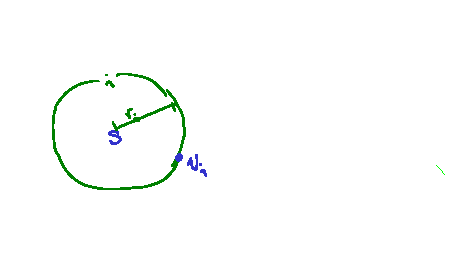
\includegraphics[width=0.75\textwidth, page=1]{figs/radius_stepping.pdf}
        }
        \only<2|handout:0>{
            \includegraphics[width=0.75\textwidth, page=2]{figs/radius_stepping.pdf}
        }
        \only<3|handout:1>{
            \includegraphics[width=0.75\textwidth, page=3]{figs/radius_stepping.pdf}
        }
        \only<4|handout:0>{
            \includegraphics[width=0.75\textwidth, page=4]{figs/radius_stepping.pdf}
        }
        \only<5|handout:1>{
            \includegraphics[width=0.75\textwidth, page=5]{figs/radius_stepping.pdf}
        }
        \only<6|handout:0>{
            \includegraphics[width=0.75\textwidth, page=6]{figs/radius_stepping.pdf}
        }
        \only<7|handout:1>{
            \includegraphics[width=0.75\textwidth, page=7]{figs/radius_stepping.pdf}
        }
    \end{center}
\end{frame}


\begin{frame}{Radius Stepping}
    \begin{algo}
        \textul{\textsc{RadiusStepping}($(1, \rho)$ graph $G = (V, E)$, source vertex $s \in V$)}: \+
        \\ $\hat{d}(\cdot) \gets  + \infty$, $\hat{d}(s) \gets 0$
        \\ $S_0 \gets \set{s}$
        \\ for $k$ from $1$ to $\ldots$
        \+ \\ $r_k \gets \min_{v \in V \setminus S_{k-1}} \set{\hat{d}(v) + r(v)}$ \-
        \+ \\ for $v_{jk} \in V \setminus S_{k-1}$ where $\hat{d}(v_{jk}) \le r_k$ \-
        \+ \+ \\ $\hat{d}(\cdot) \gets \min( \hat{d}(\cdot), \hat{d}(v_{jk}) + w(v_{jk}, \cdot) ) $ \- \-
        \\ \+ $S_k \gets \set{ v \in V \mid \hat{d}(v) \le r_k }$; $k \gets k + 1$ \-
        \\ return $\hat{d}(\cdot)$
    \end{algo}
\end{frame}

\begin{frame}{Work-Depth Tradeoffs}
    \begin{itemize}
        \pauseitem $\tilde{O}(n \rho^2 + (m + n) \rho)$ work and $\tilde{O}(\rho + \frac{n}{\rho} \log L)$ depth
        \begin{itemize}
            \pauseitem $O(n \rho^2)$ work and $O(\rho \log \rho)$ depth to preprocess
            \pauseitem $O((m + n) \rho)$ work and $O(\frac{n}{\rho} \log \rho L \log n)$ depth for Bellman-Ford
        \end{itemize}
        \pauseitem $\rho = \sqrt{n}$, then $O(\sqrt{n})$ depth, but only efficient on very dense graphs
        \pauseitem $\rho = \operatorname{polylog}(n)$, then $o(n)$ depth and nearly work efficient
    \end{itemize}
\end{frame}

\begin{frame}{SOTA}
    \begin{table}
        \begin{tabular}{ccc}
            \hline
            \textbf{Algorithm}  & \textbf{Work}         & \textbf{Span}                                              \\
            \hline
            Dijkstra            & $\tilde{O}(m)$        & $\tilde{O}(n)$                                             \\
            Bellman-Ford        & $\tilde{O}(k_n m)$    & $\tilde{O}(k_n)$                                           \\
            $\Delta^*$-Stepping & $\tilde{O}(k_n m)$    & $\tilde{O} \left( \frac{k_n (\Delta + L)}{\Delta} \right)$ \\
            Radius-Stepping     & $\tilde{O}(k_\rho m)$ & $\tilde{O} \left( \frac{k_\rho n}{\rho} \log L \right)$    \\
            $\rho$-Stepping     & $\tilde{O}(k_n m)$    & $\tilde{O} \left( \frac{k_\rho n}{\rho} \right) $          \\
            \hline
        \end{tabular}
        \caption{
            Adapted from Table 2 of \textcite{dong21-07}.
            $k_n$ is the height of shortest path tree.
            $k_\rho$ is chosen such that $G$ is a $(k_\rho, \rho)$ graph.
            $\Delta$ is a positive constant.
        }
    \end{table}
\end{frame}

\begin{frame}[allowframebreaks]{References}
    \printbibliography
\end{frame}

\end{document}
